\chapter{超材料的长通滤波器}\label{chap:5}


\section{超材料的米氏能隙和长通滤波}

\begin{figure}[!htbp]
    \centering
    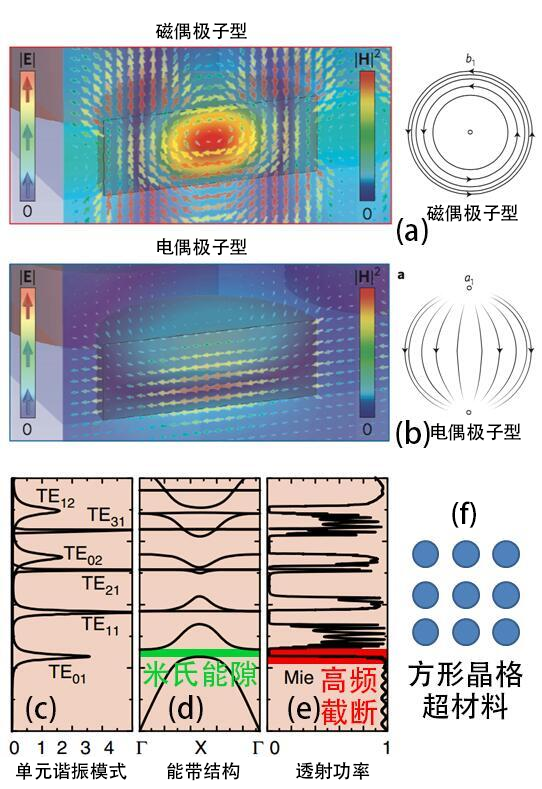
\includegraphics[width=0.9\textwidth]{Img/5-1.png}
    \caption{(a)超材料中米氏谐振分为两种主要的类型,第一种是以环形电场谐振模式的磁偶极子型谐振模式。(b) 另一种是以环形电场谐振模式的电偶极子型谐振模式。(c) 俄罗斯约飞研究所的Mikhail V. Rybin等人通过研究二维方形晶格超材料中的晶格单元的谐振模式时,计算得到的米氏谐振TE模式对应的归一化频率。(d) 通过计算布洛赫模式得到的二维方形晶格超材料的能带结构,其中最低阶的TE米氏谐振产生了米氏能隙。(e)二维方形超晶格材料的电磁波透射谱中可以看到,由于米氏能隙的存在,产生了明显的高频截断现象。(f)二维方形晶格超材料示意图,圆形阵列为高介电常数的介质材料,间隔为空气。\cite{Staude2017Metamaterial,Rybin2015Phase}}
    \label{fig:5-1}
\end{figure}
%%%%%%%%%%%%%%%%%%%%%%%%%%%%%%%%%%%%%%%%%%%%%%%%%%%%%%%%%%%%%%%%%%%%%%%%%%%%%%%%%%%%%%%%%%%%%%%%%%%%%%%%%%%%

俄罗斯约飞研究所的Mikhail V. Rybin等人的结果,通过对方形的晶格介质二维超材料进行电磁谐振模式和光子晶体带隙分析,如图5.1所示\cite{Rybin2015Phase},作者认为,当二维超材料的晶格晶格常数变得足够小或方形晶格单元的介电常数足够大的时候,二维介质超材料的电磁米氏谐振导致的米氏能隙成为最低阶的光子带隙,因而器件的布拉格衍射被抑制,米氏能隙强烈电磁响应产生的特殊电磁性质,可以用于超材料的制备和应用,如负折射、手性材料、光学隐形衣等。\cite{Zhao2009Mie,Vynck2009All,Shi2007Effects,Foteinopoulou2012Photonic,Mee2005High,Smith2000Composite,Schurig2006Metamaterial,Munk2002Frequency}

米氏谐振亚波长高折射率介质材料中一种强烈的本征电磁谐振模式,如图5.1a和5.1b,大致可以分为磁偶极子型的米氏谐振和电偶极子型的米氏谐振。其中TE偏振的入射光容易激发圆柱结构中的磁偶极子型米氏谐振,磁偶极子的产生使得材料的有效磁导率变为负数,使得光无法向前传播。

在二维介质超材料中,借助米氏谐振,如图5.1d所示的光子能带结构中,当输入光的偏振、频率在5.1d的米氏能隙频率范围内,则无法通过方形超材料区域,如图5.1e中的透射率截断现象,而当光的频率较低时(或波长较长时),则由于超材料抑制了布拉格衍射,光可以以几乎没有衍射损耗的特性,通过超材料的区域,形成明显的高频截段现象。

因此,通过超材料的米氏能隙,可以实现低布拉格衍射损耗的短波滤波功能,即实现长通滤波功能。

受自由空间的超材料米氏谐振的长通滤波的启发,认为,可以将这种特性在集成芯片上实现。


\begin{table}[!htbp]
    \caption{各种片上光子滤波器实现原理的典型指标对比}
    \label{tab:5}
    \centering
    \footnotesize% fontsize
    \setlength{\tabcolsep}{4pt}% column separation
    \renewcommand{\arraystretch}{1.2}%row space 
\begin{tabular}{ccccccc}
方案         & 特征尺寸                      & 通带宽度                 & Roll-off               & 插损dB          & 衰减dB             & Ref.         \\ \hline
环形谐振腔      & \textgreater{}10×10 $\mu$m$^2$   & \textless 5nm        & \textgreater{}50dB/nm  & \textless 1   & \textgreater 40  & \cite{Optical2006,Bogaerts2015Silicon} \\
马和曾德尔干涉仪   & \textgreater{}50×50 $\mu$m$^2$   & \textgreater{}10nm   & \textgreater{}10 dB/nm & \textless{}1  & 15-20            &\cite{Chen2017Silicon}   \\
阵列波导光栅     & \textgreater{}500×500 $\mu$m$^2$ & \textless 5 nm       & \textgreater{}50dB/nm  & \textless{}3  & \textgreater{}25 & \cite{Daoxin2011Low}   \\
布拉格光栅/光子晶体 & \textgreater{}10×10 $\mu$m$^2$   & \textgreater{}50nm   & \textless{}1 dB/nm     & \textless 0.5 & $\sim$20         & \cite{Jiang2011Slab}    \\
频谱选择波导     & \textgreater{}3×100 $\mu$m$^2$   & \textgreater{}1000nm & 2.82 dB/nm             & \textless{}1  & 15-20            & \cite{Magden2018Transmissive}    \\
超材料响应      & $\sim$5×5$\mu$m$^2$              & 50nm                 & 0.493 dB/nm            & $\sim$0.5     & $\sim$25         & 本论文       
\end{tabular}
\end{table}
%%%%%%%%%%%%%%%%%%%%%%%%%%%%%%%%%%%%%%%%%%%%%%%%%%%%%%%%%%%%%%%%%%%%%%%%%%%%%%%%%%%%%%%%%%%%%%%%%%%%%%%%%%%%
%%%%%%%%%%%%%%%%%%%%%%%%%%%%%%%%%%%%%%%%%%%%%%%%%%%%%%%%%%%%%%%%%%%%%%%%%%%%%%%%%%%%%%%%%%%%%%%%%%%%%%%%%%%%
%%%%%%%%%%%%%%%%%%%%%%%%%%%%%%%%%%%%%%%%%%%%%%%%%%%%%%%%%%%%%%%%%%%%%%%%%%%%%%%%%%%%%%%%%%%%%%%%%%%%%%%%%%%%

在片上的光滤波,在通信、传感和非线性中具有广泛应用。如表5-1所示,分析了现有片上光子滤波器,通过对比现有的光子滤波原理去实现类似的长通滤波功能。通过对比,认为超材料的米氏响应,可以在极其紧凑的器件尺寸下,实现较为满意的长通滤波特性,有利于光子芯片的高度集成。

\section{超材料长通滤波器器件}

\begin{figure}[!htbp]
    \centering
    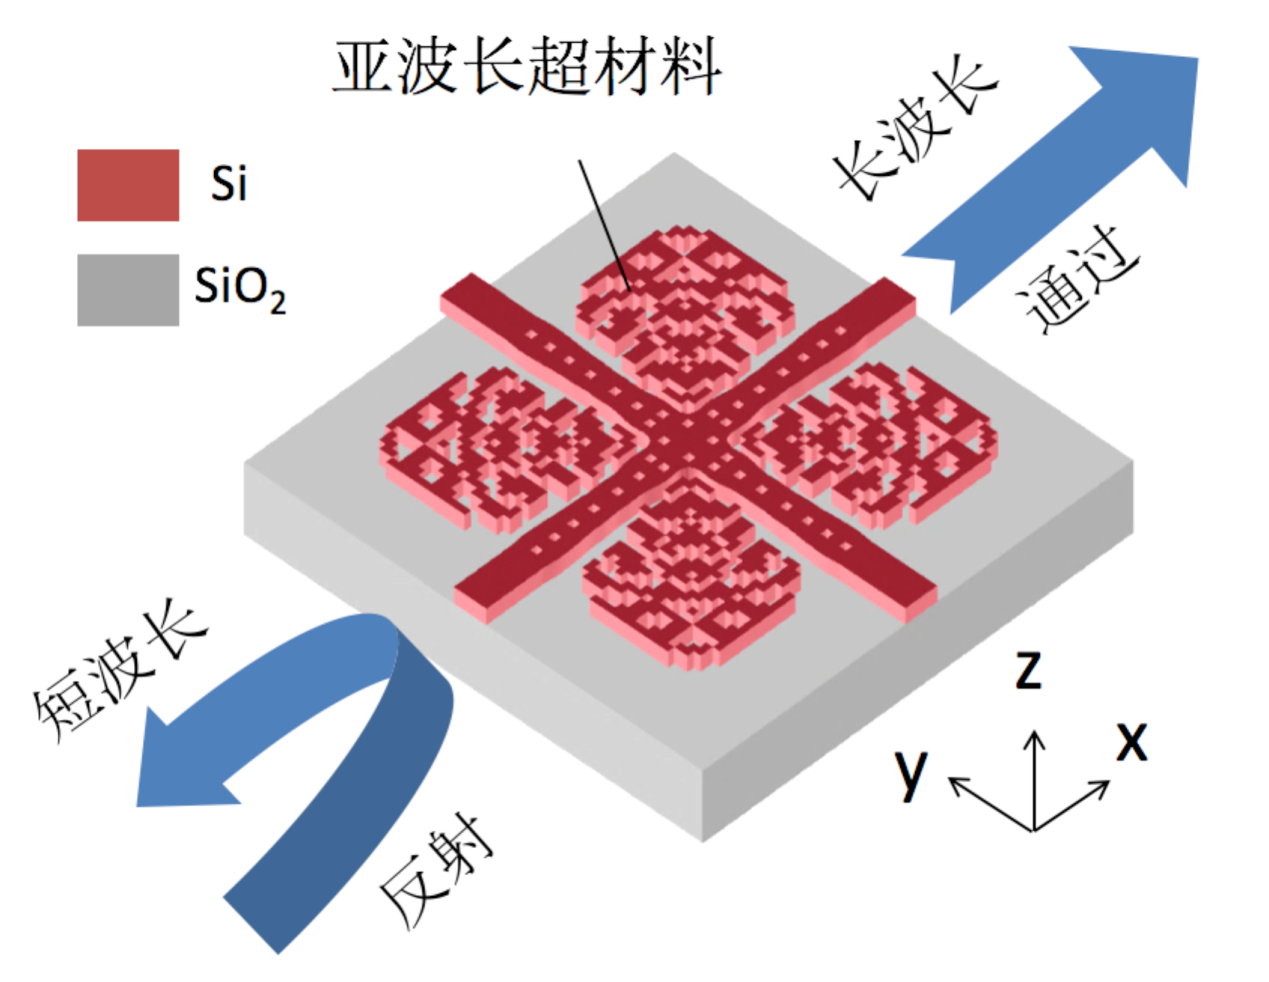
\includegraphics[width=1\textwidth]{Img/5-2.png}
    \caption{超材料长通滤波器的概念图,其中滤波器由一个与单模硅波导相连的亚波长的超材料组成。其中短波长的光,由于超材料结构的电磁响应而不能通过,反射回原波导中。而长波导的光由于偏离了超材料的电磁响应频率,可以通过亚波长的超材料区域。}
    \label{fig:5-2}
\end{figure}
%%%%%%%%%%%%%%%%%%%%%%%%%%%%%%%%%%%%%%%%%%%%%%%%%%%%%%%%%%%%%%%%%%%%%%%%%%%%%%%%%%%%%%%%%%%%%%%%%%%%%%%%%%%%


受超材料米氏响应的长通滤波特性的启发,设计了一个片上的亚波长的超材料光子器件结构,其超材料器件结构如图5.2所示,以实现片上的超材料长通滤波功能。其中长通滤波器由一个与波导连接的亚波长超材料组成,可以通过一步的等离子体刻蚀实现制备。光从波导输入到超材料结构区域时,其中长波长的光,可以无视超材料的亚波长结构而直接通过,而短波长的光,则由于超材料的强烈的电磁模式响应,不能通过超材料区域,被器件结构反射。由于长通滤波器的波导集成特性,尺寸紧凑,可以实现更高的集成度,在实际应用中具有较高的应用价值。

有了超材料长通滤波器的器件概念后,器件的设计的重点在于设计超材料的结构部分,已实现所需的滤波功能。

\begin{figure}[!htbp]
    \centering
    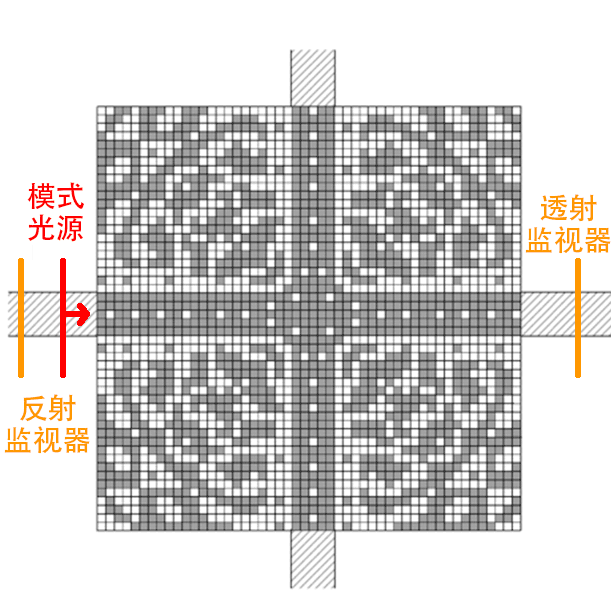
\includegraphics[width=1\textwidth]{Img/5-3.png}
    \caption{超材料长通滤波器的优化第一步,通过遗传算法优化的二值化的像素图案,其中每个像素的尺寸为100×100nm,黑色像素代表了高折射率的硅,白色像素代表低折射率的空气。}
    \label{fig:5-3}
\end{figure}
%%%%%%%%%%%%%%%%%%%%%%%%%%%%%%%%%%%%%%%%%%%%%%%%%%%%%%%%%%%%%%%%%%%%%%%%%%%%%%%%%%%%%%%%%%%%%%%%%%%%%%%%%%%%


如图5.3所示,将设计超材料光子滤波器的超材料结构部分。第一步,优化了一个像素图案结构。希望最终的器件的尺寸在5×5$\mu$m$^2$的占地面积,因此图中仿真的超材料区域划分为51×51个单元格,其中每个单元格的尺寸为100×100×220nm(长×宽×高),可以通过商用的标准SOI晶片实现制备。超材料的结构的下方是二氧化硅氧化层,如图5.2所示,而由于超材料光子器件通常需要较大的折射率反差来实现较好的电磁谐振响应,因此结构的上方采用空气来实现较大的折射率反差。通过像素结构的图案的黑白组合,黑色像素代表硅,白色像素代表空气,来实现长通滤波的功能。

并通过Lumerical的脚本环境,结合遗传算法的变量优化,来实现像素图案的优化。

在遗传算法优化设计过程中,为减少算法优化的时间,采取了4轴折叠对称的结构,如图5.4a,使得需要独立优化的单元的个数减少为351个,为原来的1/8,另外,保持高度的对称性,使长通滤波的响应频率可以随着器件版图的缩放而发生平移。

通过四轴折叠对称之后,如图5.4b所示,所有的二值化的独立变量的个数一共有351个。如图5.4c所示的遗传算法优化程序框图,在351个二值的独立变量的优化中,优化了1550nm的S21参数和1450nm的S11参数。
 
假定了左端波导为端口1而右端波导为端口2,其中S21参数为从左端波导中输入的光信号时,在右端的光波导收集到的光功率。而S11参数为从左端波导中输入光信号时,从超材料左端波导反射回去的功率。

\begin{figure}[!htbp]
    \centering
    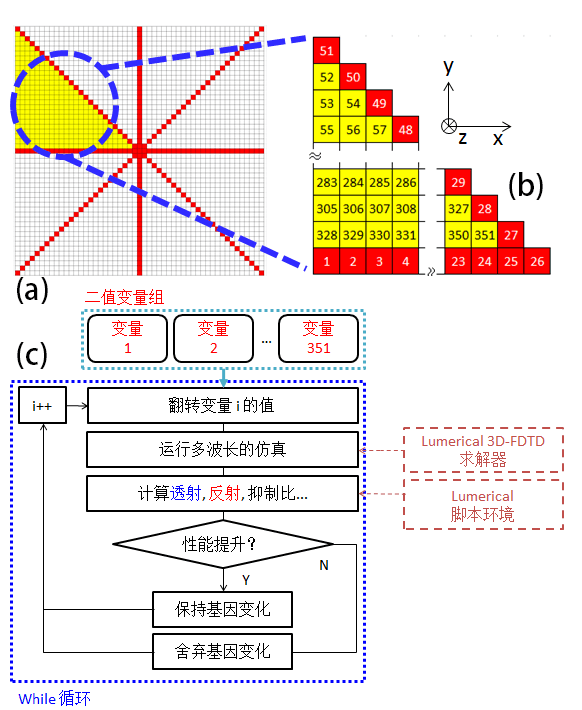
\includegraphics[width=1\textwidth]{Img/5-4.png}
    \caption{(a)在遗传算法优化超材料像素图案过程中,通过四轴折叠对称,可以得到需要独立优化的变量个数仅为像素图案的八分之一。(b) 351个独立的像素变量分布示意图。(c)通过对351个二值化变量进行遗传算法优化,可以得到最终的超材料像素图案如图5.5所示。}
    \label{fig:5-4}
\end{figure}
%%%%%%%%%%%%%%%%%%%%%%%%%%%%%%%%%%%%%%%%%%%%%%%%%%%%%%%%%%%%%%%%%%%%%%%%%%%%%%%%%%%%%%%%%%%%%%%%%%%%%%%%%%%%

\begin{figure}[!htbp]
    \centering
    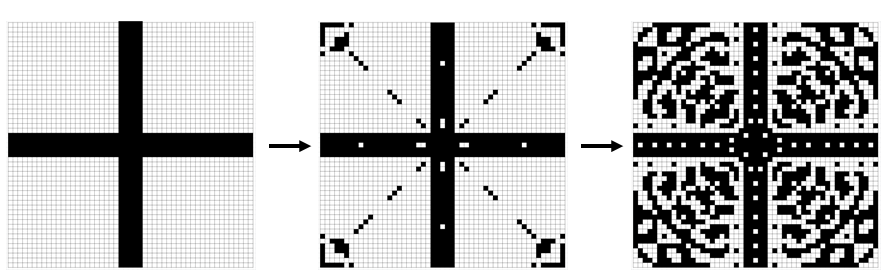
\includegraphics[width=1\textwidth]{Img/5-5.png}
    \caption{遗传算法的优化过程,算法的优化从一个简答你的四轴折叠对称的普通光交叉开始,逐步变化像素点的结构分布,最终形成超材料的像素结构。}
    \label{fig:5-5}
\end{figure}
%%%%%%%%%%%%%%%%%%%%%%%%%%%%%%%%%%%%%%%%%%%%%%%%%%%%%%%%%%%%%%%%%%%%%%%%%%%%%%%%%%%%%%%%%%%%%%%%%%%%%%%%%%%%

随着Lumerical遗传算法优化程序的进行,如图5.5所示,器件的仿真从一个简单的十字波导交叉开始,不断修正像素图的结构,并最终得到了一个具有长通滤波特性的像素图案。
 
经过上述的像素图案的优化后,经过Lumerical 3D-FDTD验算得到的长通滤波器在1550nm的S21插入损耗约为-0.5dB,而1450nm的 S21插入损耗约为-20dB,其短波长的截段的特性较为明显,然而其1550nm处的长通波段的S21插入损耗较大,因此,考虑第二步的优化,进一步提升器件在长通波段的S21参数指标。

\begin{figure}[!htbp]
    \centering
    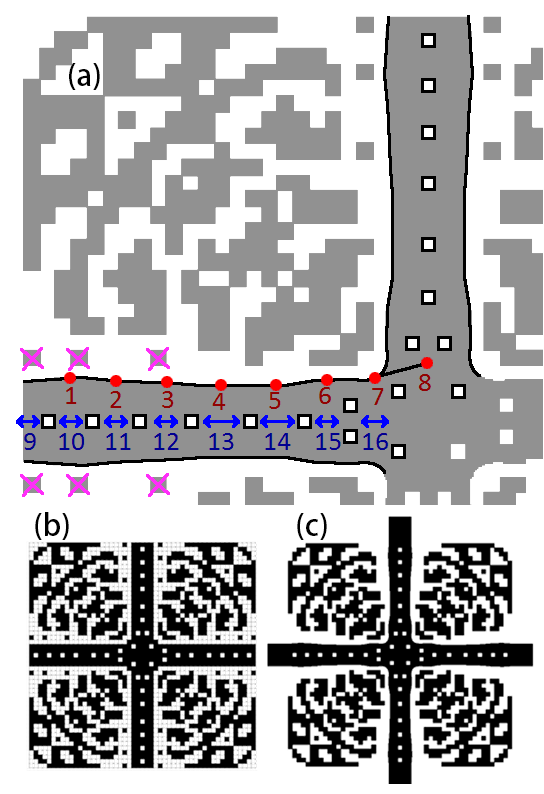
\includegraphics[width=0.8\textwidth]{Img/5-6.png}
    \caption{长通滤波器设计的遗传算法优化第二步。(a)通过优化中间波导上的波导剖面宽度和中间的方形孔的位置,通过优化8个波导剖面宽度和8个挖孔位置变量,减少在长通波段下的插入损耗,增大器件的性能。(b)第二步优化之前的像素点结构图。(c)优化了波导剖面宽度和挖孔位置后的超材料结构示意图。}
    \label{fig:5-6}
\end{figure}
%%%%%%%%%%%%%%%%%%%%%%%%%%%%%%%%%%%%%%%%%%%%%%%%%%%%%%%%%%%%%%%%%%%%%%%%%%%%%%%%%%%%%%%%%%%%%%%%%%%%%%%%%%%%

如图5.6b和5.6c所示,在器件优化的第二步中,主要考虑优化中间波导的波导剖面形状和挖孔的位置,通过优化上述,进一步的降低器件在长通波段的插入损耗,使得器件的S21插入损耗更低。
 
如图5.6a所示,进一步优化波导的剖面形状和挖孔位置作为变量,一共有16个新引入的位置变量,16个变量通过遗传算法进行优化,实现更低的通带损耗,优化后的长通滤波器的结构如图5.6c所示。

\begin{figure}[!htbp]
    \centering
    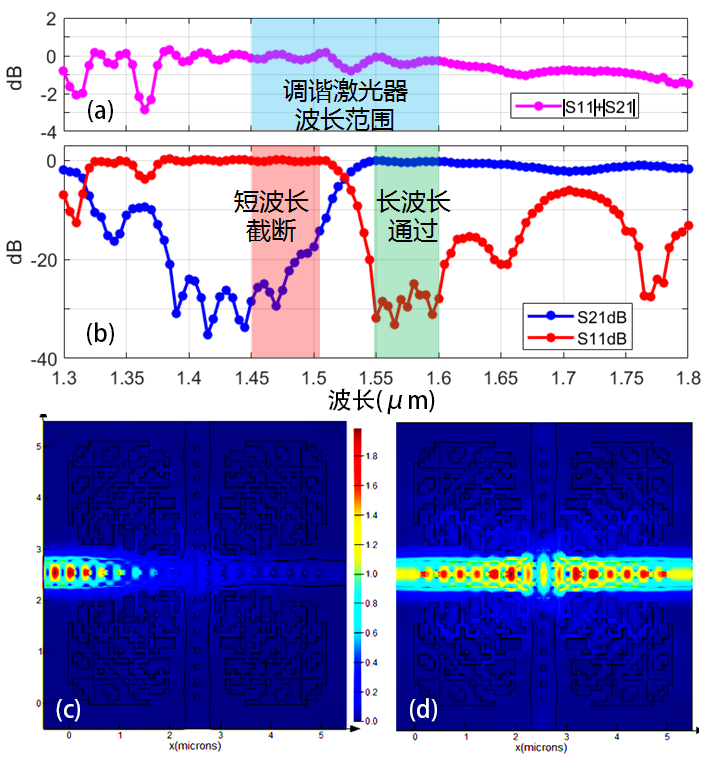
\includegraphics[width=1\textwidth]{Img/5-7.png}
    \caption{经过两步优化的超材料长通滤波器的波长响应仿真结果图。(a) 3D-FDTD仿真得到的不同波长下|S11|+|S21|结果,可见由于超材料的亚波长特征尺寸,器件的布拉格衍射受到抑制,总功率大致保持守恒。 (b) 仿真得到的S21dB透射谱和S11dB反射谱,可见,在1450-1500nm左右,短波长的光被全部反射,而在1550-1600nm波长的光,则可以通过超材料区域。(c)当通入波长为1450nm的TE模式时,由于超材料区域的强烈电磁响应而被反射回原波导中。(d) 当通入波长为1550nm的TE模式时,由于没有激发超材料的谐振模式,光可以通过超材料区域。}
    \label{fig:5-7}
\end{figure}
%%%%%%%%%%%%%%%%%%%%%%%%%%%%%%%%%%%%%%%%%%%%%%%%%%%%%%%%%%%%%%%%%%%%%%%%%%%%%%%%%%%%%%%%%%%%%%%%%%%%%%%%%%%%

在经过了上述的两步优化之后,通过Lumerical 3D-FDTD中对器件的性能进行详细的仿真,如图5.7c和5.7d所示,从波导端口1输入1450nm和1550nm的TE基础模式光,可以发现1450nm波长的光不能通过超材料区域,而1550nm的光可以通过。

通过Lumerical扫描S11和S21参数随波长变化的变化情况,如图5.7b所示,其中,1.45$\mu$m$\sim$1.6$\mu$m为实验室的激光器8164B所能调谐的波长范围,从仿真的波长响应结果来看,在1.45$\mu$m$\sim$1.5$\mu$m的范围为器件的截止波段,由于超材料的电磁响应,TE模式的光的米氏谐振导致介质有效磁导率变为负数,使得光不能通过,且短波截断的功率衰减为$\sim$25dB,在1.55$\sim$1.6$\mu$m为长通波段,其仿真得到的1550nm处的理论插入损耗为-0.1dB。

而且,在1.45$\mu$m$\sim$1.6$\mu$m波段,总的$|S11|+|S21|$功率的总和保持功率守恒,意味着由于超材料的亚波长特性,超材料区域的衍射损耗几乎被抑制,如图5.7a所示。

\begin{figure}[!htbp]
    \centering
    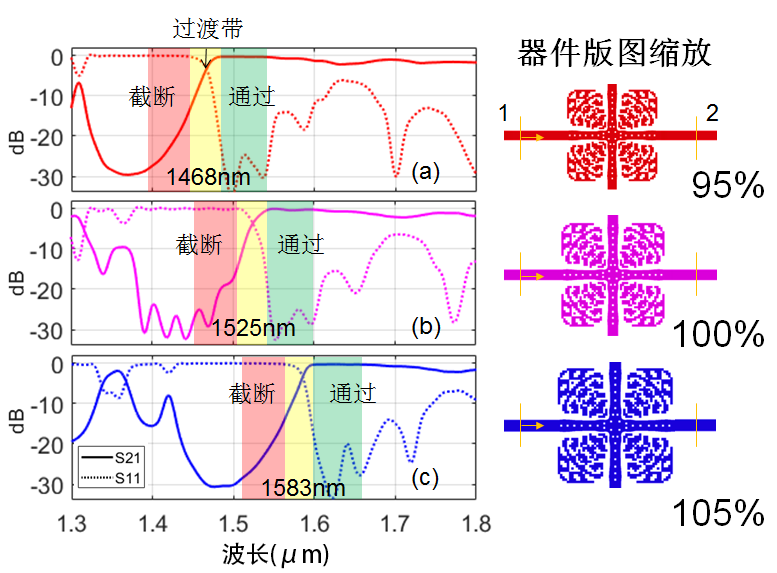
\includegraphics[width=1\textwidth]{Img/5-8.png}
    \caption{超材料长通滤波器的滤波特性与器件版图的缩放关系。(a)当器件版图缩放为原尺寸的95\%时的波长响应。(b)当器件版图为100\%原尺寸时的波长响应。(c) 当器件版图缩放为原尺寸的105\%时的波长响应。可见随着器件版图的缩放,过渡带对应的波长会发生明显的偏移,偏移的程度为11.4nm/1\%。}
    \label{fig:5-8}
\end{figure}
%%%%%%%%%%%%%%%%%%%%%%%%%%%%%%%%%%%%%%%%%%%%%%%%%%%%%%%%%%%%%%%%%%%%%%%%%%%%%%%%%%%%%%%%%%%%%%%%%%%%%%%%%%%%

在上述超材料长通滤波器设计中,通过激发超材料结构中的电磁响应实现长通滤波的功能,因此,通过改变超材料结构的电磁响应频率,则改变器件的截止波段。

而最直观简单的改变响应频率的方法,可以通过器件版图的缩放来实现。如图5.8所示,通过对器件的版图施行缩放,尝试了95\%、100\%和105\%不同的缩放比例。在Lumerical中,对缩放后的长通滤波器的S11和S21参数进行扫描,通过波长扫描,得到了图5.8中波长响应的结果,当器件的版图缩放时,器件的长通滤波功能仍然有效,截断的抑制比保持20dB以上,而器件的短波截断和长波通过波段会发生整体平移。当器件的缩放尺寸为95\%时,器件的过渡带的中心波长为1468nm,当器件的缩放尺寸为105\%时,器件的过渡带的中心波长为1583nm。器件的缩放尺寸每缩放1\%,则过渡带的中心波长则相应地平移11.4nm。

上述的仿真结果表明,可以通过简单的器件版图缩放来改变超材料结构的电磁响应频率,从而改变长通滤波的截止波段和长通波段的位置。

\begin{figure}[!htbp]
    \centering
    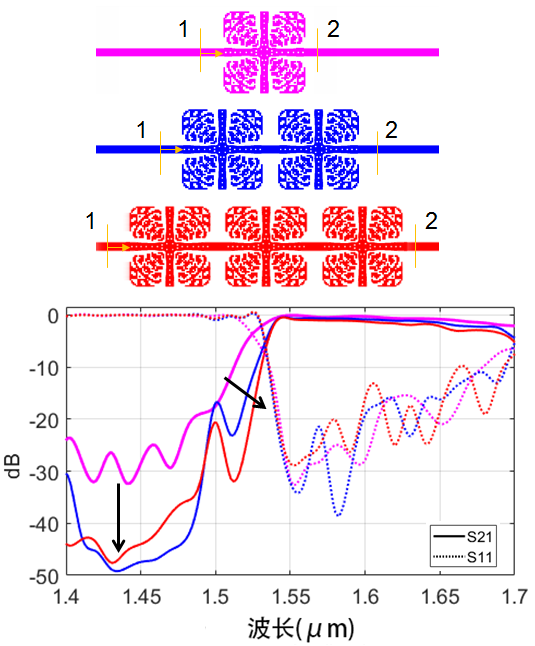
\includegraphics[width=1\textwidth]{Img/5-9.png}
    \caption{超材料长通滤波器的滤波特性与器件级联的关系。通过1、2、3个长通滤波器之间级联,实现了过渡带斜率的增强。}
    \label{fig:5-9}
\end{figure}
%%%%%%%%%%%%%%%%%%%%%%%%%%%%%%%%%%%%%%%%%%%%%%%%%%%%%%%%%%%%%%%%%%%%%%%%%%%%%%%%%%%%%%%%%%%%%%%%%%%%%%%%%%%%

另一方面,对于长通滤波器,尝试通过器件级联的方法来改变中间的过渡带的宽度。


如图5.9所示,尝试了不同级联个数的器件,如1,2,3个级联,通过Lumerical仿真得到的不同个数的器件的S11和S21参数,可以看到,随着器件的级联个数的增加,器件的短波波段的滤波功率衰减越来越大,达到了-40dB以上,而在长通波段,其插入损耗S21并没有明显增大,在长通波段的反射也能很好的保持在-20dB以下。最主要的,其过渡带的斜率随着器件级联个数的增加而明显的变大,更陡峭的过渡带斜率,在片上滤波应用上具有重要意义。

上述的仿真结果表明,可以通过简单的器件版图级联,来实现长通滤波的过渡带斜率的调节。

\section{超材料长通滤波器的制备与测试}

\begin{figure}[!htbp]
    \centering
    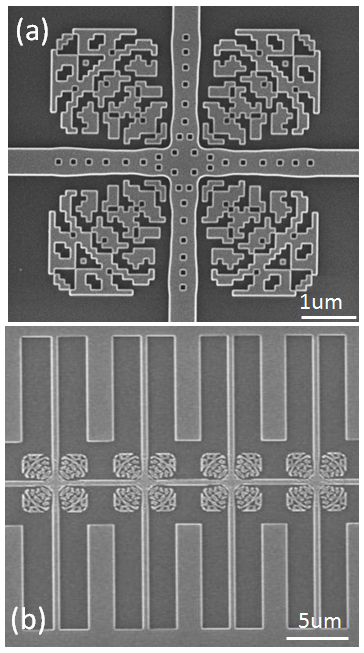
\includegraphics[width=0.6\textwidth]{Img/5-10.png}
    \caption{ (a)加工后的超材料长通滤波器在电子显微镜下的结果。(b)加工后的级联超材料长通滤波器。}
    \label{fig:5-10}
\end{figure}
%%%%%%%%%%%%%%%%%%%%%%%%%%%%%%%%%%%%%%%%%%%%%%%%%%%%%%%%%%%%%%%%%%%%%%%%%%%%%%%%%%%%%%%%%%%%%%%%%%%%%%%%%%%%

通过器件制备和测试来验证仿真的结果。器件的制备过程相对简单,只需在标准的SOI晶片上通过单次的电子束曝光和等离子体刻蚀便可以实现器件制备,如图5.10a为加工后的长通滤波器在电子显微镜SEM下的结果,同时也制备了不同级联个数的器件,如图5.10b,用于测试器件的级联特性和缩放特性。

\begin{figure}[!htbp]
    \centering
    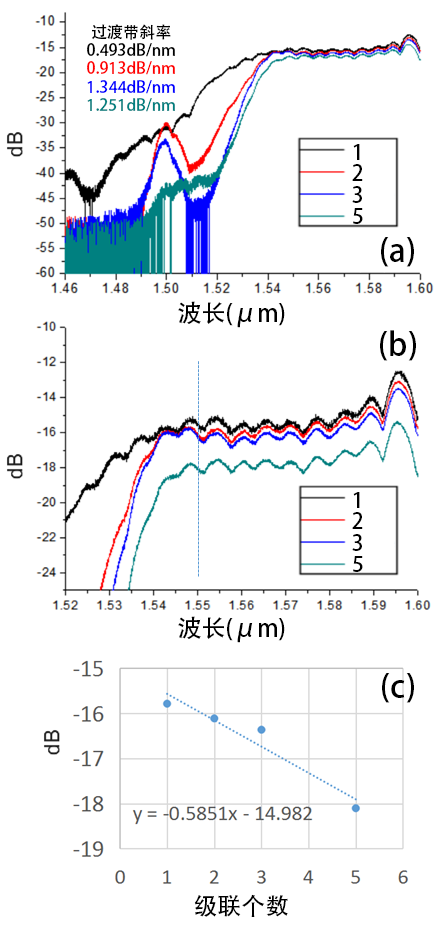
\includegraphics[width=0.7\textwidth]{Img/5-11.png}
    \caption{长通滤波器的级联测试结果图。(a)在1,2,3,5不同级联个数下,测试得到的投射谱,对应的过渡带斜率为0.493,0.913,1.344,1.251dB/nm。(b) 在1,2,3,5不同级联个数下,长通波段的透射功率。可以通过提取长通波段的透射功率,通过线性拟合的方式,得到长通波段的插入损耗。(c)通过提取1550nm处的透射功率,并通过线性拟合得到,单个长通滤波器的插入损耗约为-0.5851dB@1550nm。}
    \label{fig:5-11}
\end{figure}
%%%%%%%%%%%%%%%%%%%%%%%%%%%%%%%%%%%%%%%%%%%%%%%%%%%%%%%%%%%%%%%%%%%%%%%%%%%%%%%%%%%%%%%%%%%%%%%%%%%%%%%%%%%%

\begin{figure}[!htbp]
    \centering
    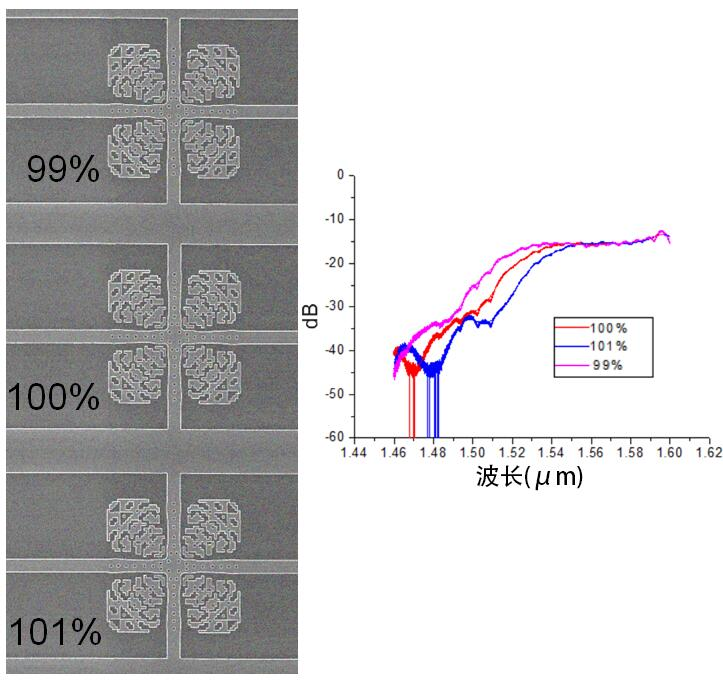
\includegraphics[width=1\textwidth]{Img/5-12.png}
    \caption{长通滤波器的版图缩放测试结果图。可见,随着器件版图缩放1\%时,器件的透射谱偏移了10nm左右,与仿真结果较为一致。}
    \label{fig:5-12}
\end{figure}
%%%%%%%%%%%%%%%%%%%%%%%%%%%%%%%%%%%%%%%%%%%%%%%%%%%%%%%%%%%%%%%%%%%%%%%%%%%%%%%%%%%%%%%%%%%%%%%%%%%%%%%%%%%%

加工后的器件的测试结果,同样采用了间接测试的方案。测试了1,2,3,5个器件的光纤到光纤的透射谱,如图5.11a所示。通过对比不同的测试结果,间接地得到单个器件的测试结果。
通过不同器件个数下光纤到光纤的透射谱,从投射谱可看到较为明显的长通滤波现象,而且,随着器件级联个数的增加,其过渡带宽度逐渐变小,过渡带的斜率也逐渐增大。
其对应的过渡带的斜率依次为0.493,0.913, 1.344, 1.251 dB/nm。
禁带的功率抑制比也逐渐增大,然而由于无法避免的TM模式的存在,其短波长的功率抑制无法达到仿真的水平,维持在30dB的量级。
而对于长通波段的插入损耗,可以通过线性拟合的方式得到。
如图5.11c所示,通过线性拟合如图5.11a中,在1550nm处的器件插入损耗,可得到单个长通滤波器在1550nm处的损耗为-0.58dB。

同样,为了测试器件在不同的缩放情况下的光通过情况,如图5.12所示,测试了99\%,100\%和101\%缩放的器件,其测试得到的光纤到光纤透射谱中,可以看到,当器件缩放1\%时,禁带的位置偏移了10nm,与仿真的结果的11.4nm较为一致。

\section{小结}

在本章中,设计并加工了一个紧凑的超材料长通滤波器,器件尺寸仅为 5.1×5.1$\mu$m$^2$。在长通滤波器的长通波段(1550$\sim$1600nm),器件的插入损耗仅为-0.58dB。而在短波长截止波段(约1450$\sim$1500nm),光会由于超材料结构的电磁响应而被过滤并反射,且功率衰减可以达到25dB。我们同样展示了长通滤波器的由于器件版图缩放导致的过渡带偏移现象和由器件级联带来的过渡带斜率增强现象。这些实验结果表明,超材料可以成为一种紧凑而理想的设计方法,用来实现片上的滤波功能,对于提高光子器件的集成度和降低光子集成芯片成本,具有积极的意义。

